\chapter{はじめに}
\thispagestyle{myheadings}

\section{背景}
人の歌声や喋り声を人工的に再現する音声合成ソフトは数多く存在しており,それらソフトのほとんどが複数種類の声を切り替えて使用できる.
また,その中でもいくつかのソフトでは個人が声の元となる合成音声ライブラリを作成し,第三者による利用を前提とした配布を行える.
例えば,喋り声を対象とした合成音声ソフトCOEIROINKではユーザの作成した音声合成モデルが350キャラクタ分以上配布されているほか\cite{mycoeiroink},歌声を対象とした合成音声ソフトUTAUでは同ソフト上で使用できるUTAU音源ライブラリが7000キャラクタ分以上存在する\cite{vdbutau}.
このように,今や合成音声ソフトの利用者は使える声に対し非常に多くの選択肢を持っており,その全ての把握は現実的ではない.

合成音声を利用するシーンにおいて,声が持つイメージや印象は声を選ぶ上で考慮すべき要素である.
例えば喋らせるアナウンスの内容や,歌わせる曲調など用途に合った声質を持つライブラリを選択し,用いるのは制作において重要なプロセスである.
しかし,現状声の持つ印象を知るには実際に聴いてみるのが最も有力な手段であり,数多あるライブラリの生み出す声を十分な数聴き比べ適切な声を採択するには多大な手間と時間を要する.
その結果として,ユーザがライブラリを選ぶ際,その多くが普段の生活の中で聞いた経験のある声や,知っているキャラクターの声を選択していると考えられる.
これはユーザ全体の中で使われる声に大きな偏りを生じさせてしまう.
万に近い数存在するライブラリのうち実際にユーザに用いられる声は一握りであり,ほとんどのライブラリはユーザに用いられず埋もれてしまう.

\section{研究目的とアプローチ}
そこで本研究では,ライブラリごとの声に対する印象を事前に数値化し,それを用いてユーザの求める声に近いライブラリを探索するサービスを提案する.
探索対象とする合成音声ソフトは特に利用できるライブラリが多く,後述する声質に関するアンケートが存在しているUTAU音源ライブラリを対象とする.
本サービスでは事前に,声に対する印象を複数の印象軸ごとに評価スコアとして数値化する.
ユーザは理想としてイメージする声の評価スコアを入力し,目的に合った音源を探索できる.
評価スコアの軸には,例えばスコアの高低を女性らしい声・男性らしい声に対応させた"性別感"など,ユーザが声からスコアを,あるいはスコアから声をある程度想定できるような直感的な軸が望ましい.
各音源に対する評価スコアは,アンケート調査によって集められたデータをもとに音源ファイルから各評価スコアを推定できる機械学習モデルを作成し,それを用いて付与する.
また,本サービスは多くの人が手軽に利用できるようWebサービスとして実装する.

\begin{figure}[h]
  \centering
  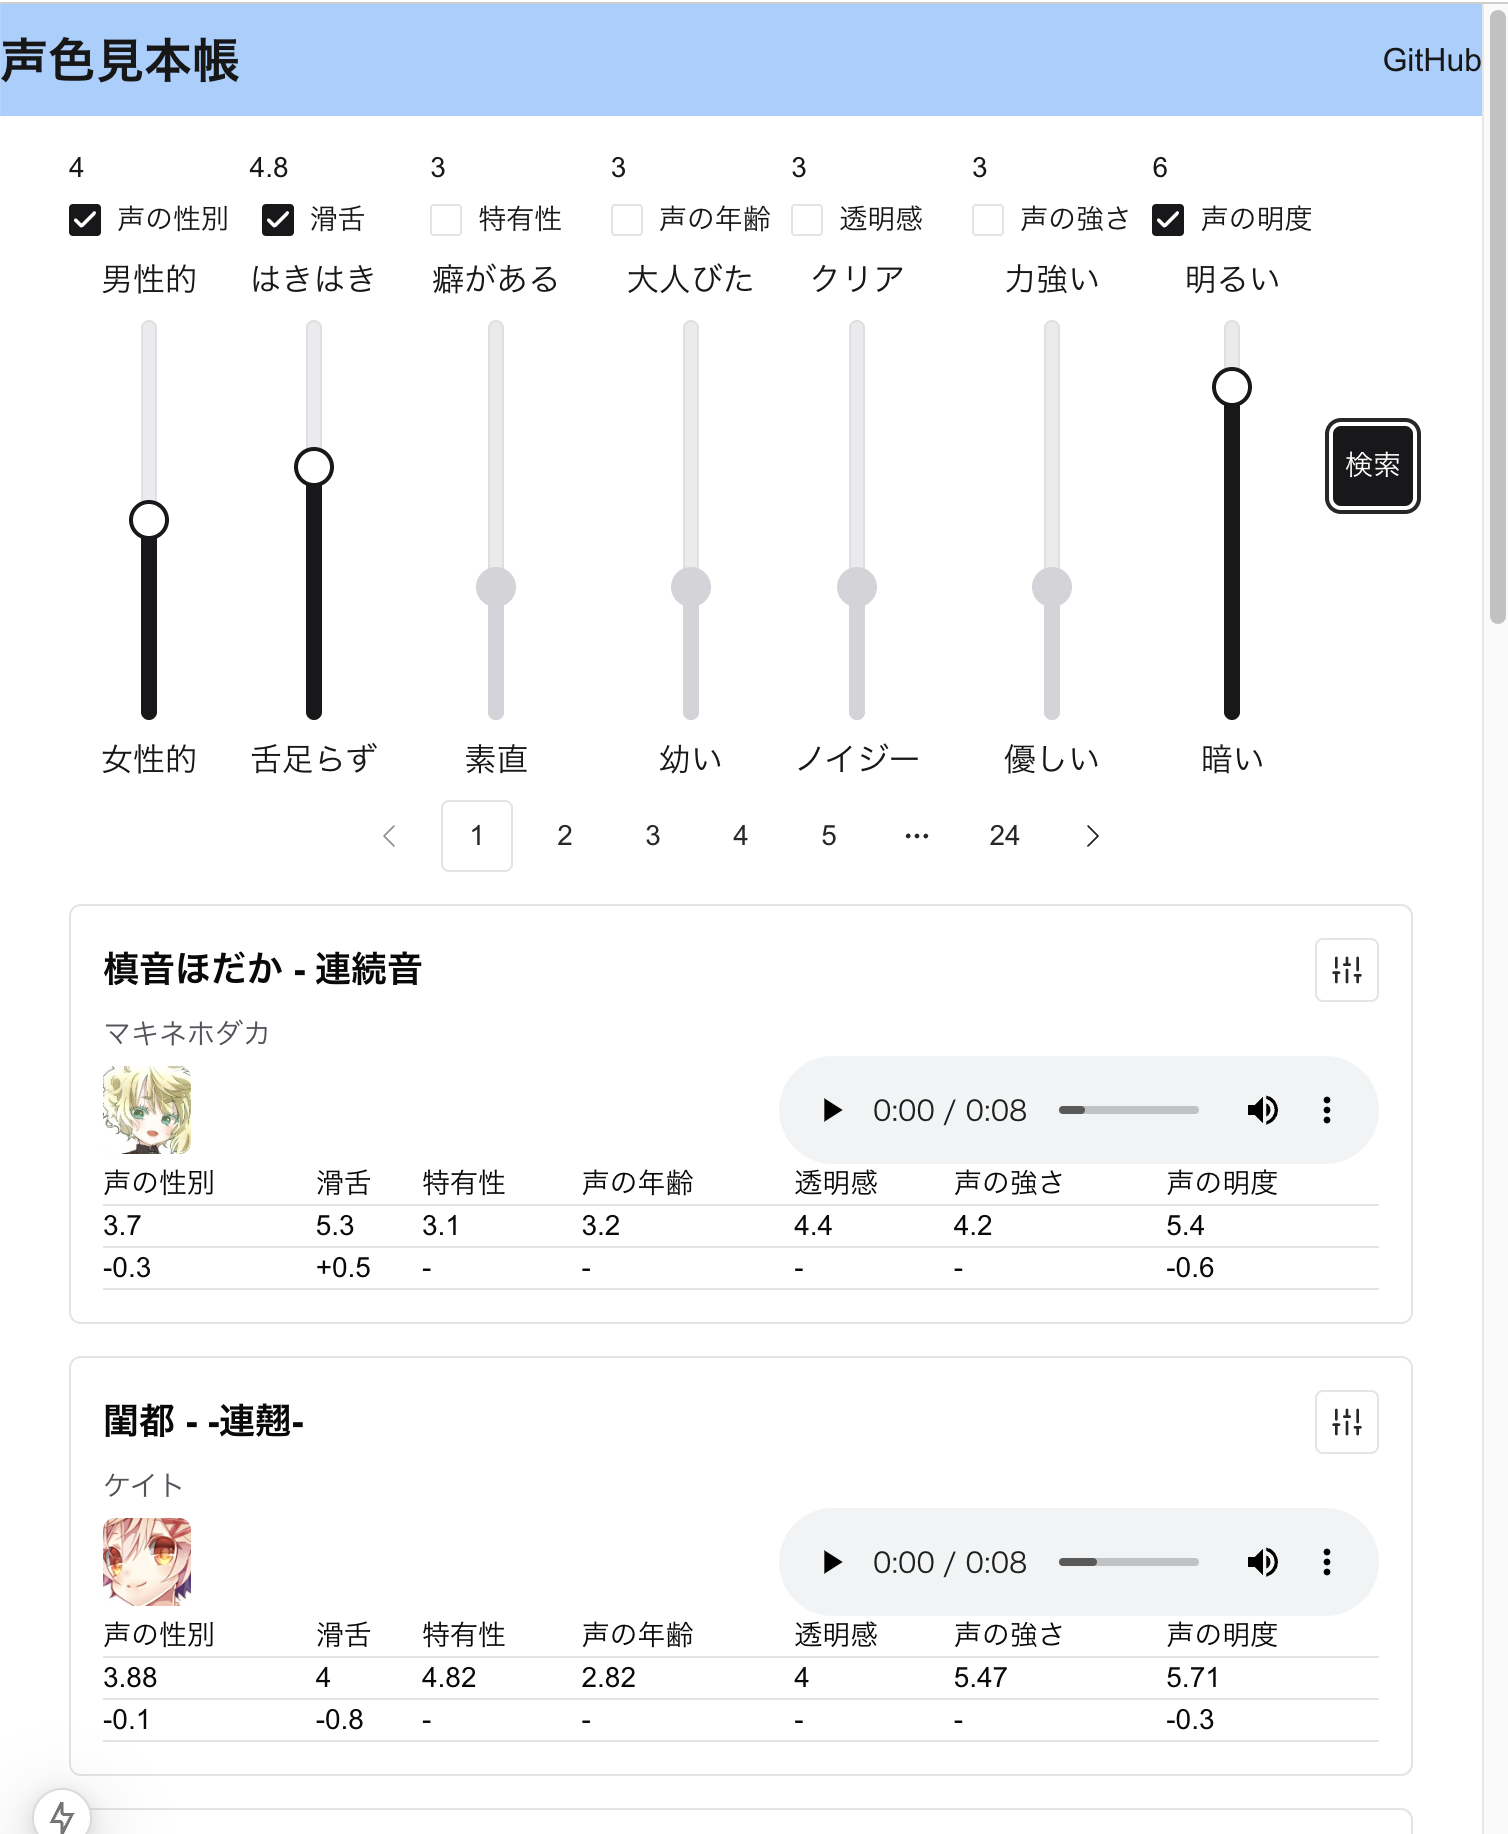
\includegraphics[width=0.9\linewidth]{fig/site_image.png}
  \caption{サービスの画面イメージ}
  \label{fig:site_image}
\end{figure}

\section{本論文の構成}

% Local Variables:
% mode: japanese-LaTeX
% TeX-master: "root"
% End:
